\cleardoublepage
\chapter{ANALISIS}
\label{chap:analisis-masalah}

Bab ini memaparkan analisis kondisi pengelolaan diabetes melitus tipe 1 yang berlaku saat ini, analisis kebutuhan sistem yang diusulkan, analisis data dan metodologi yang mendasarinya, serta analisis pemilihan solusi beserta justifikasinya. Bab ini merupakan realisasi aktivitas kedua pada kerangka DSRM, yaitu perumusan tujuan solusi, sebagaimana dipaparkan pada Subbab~\ref{sec:metodologi-penelitian}. Keputusan yang dihasilkan pada bab ini menjadi masukan langsung bagi perancangan pada Bab~\ref{chap:perancangan}.

\section{Analisis Kondisi Saat Ini}
\label{sec:kondisi-saat-ini}

\subsection{Model Konseptual Alur Perawatan}
\label{subsec:model-konseptual}

Pengelolaan DMT1 di Indonesia berjalan melalui alur yang berbeda dari pengelolaan diabetes tipe 2. Diagnosis awal kerap terjadi pada keadaan gawat, karena kesadaran mengenai DMT1 yang masih rendah di kalangan masyarakat maupun tenaga kesehatan menyebabkan banyak pasien baru dikenali setelah mengalami ketoasidosis diabetik \autocite{pulungan2021}. Setelah diagnosis ditegakkan, pengelolaan berlanjut melalui layanan rujukan yang ditangani dokter spesialis, bukan melalui layanan primer sebagaimana lazimnya penyakit kronis lain \autocite{faizi2025}.

Alur perawatan yang berlaku dapat digambarkan sebagai interaksi antara lima komponen. Komponen pertama adalah pasien beserta keluarga, yang menjalankan pemantauan glukosa mandiri melalui tusuk jari dan mencatatnya pada \emph{logbook} secara periodik. Komponen kedua adalah catatan \emph{logbook} itu sendiri, yang menjadi satu-satunya rekaman kondisi glikemik di antara dua kunjungan. Komponen ketiga adalah kunjungan kontrol berkala, yang menjadi titik temu antara pasien dan dokter. Komponen keempat adalah dokter spesialis yang menafsirkan catatan tersebut secara manual pada saat kunjungan. Komponen kelima adalah pedoman klinis yang dirujuk dokter untuk menetapkan penyesuaian terapi. Alur kerja kelima komponen tersebut ditunjukkan pada Gambar~\ref{fig:alur-perawatan}.

\begin{figure}[htbp]
\centering
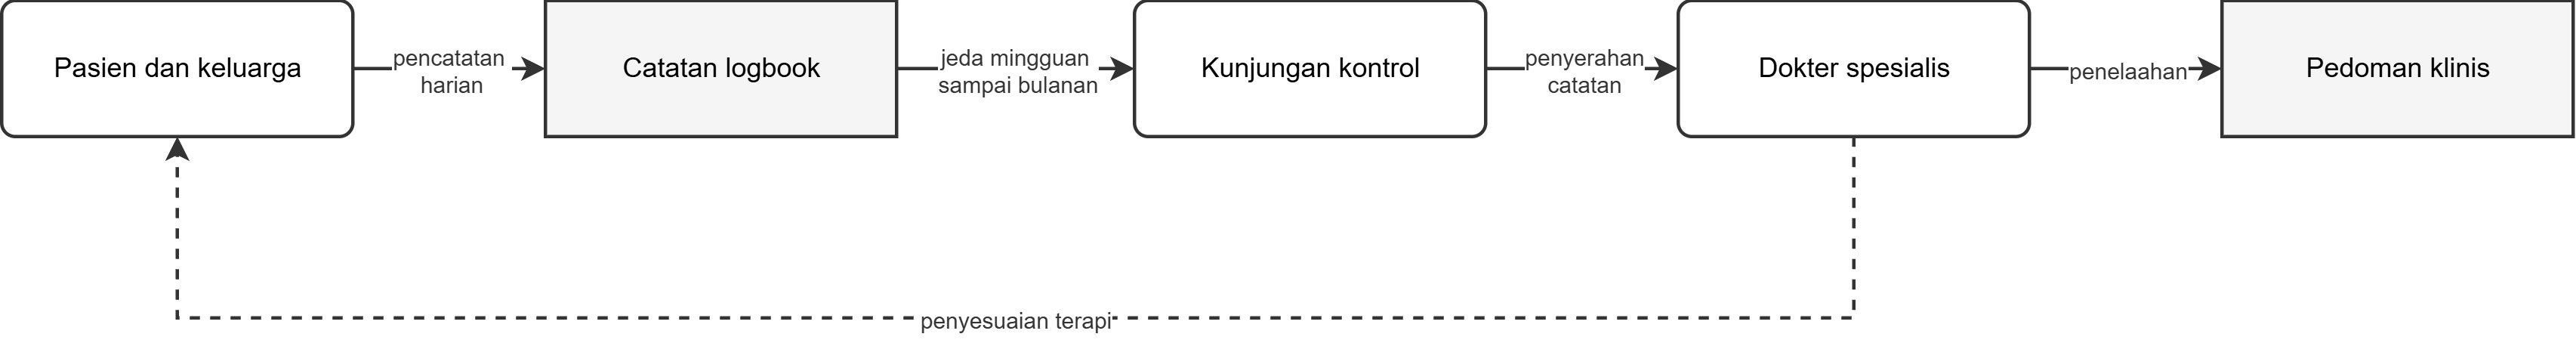
\includegraphics[width=0.95\textwidth]{images/Gambar_III1_AlurPerawatanDMT1.png}
\caption{Model konseptual alur perawatan DMT1 saat ini.}
\label{fig:alur-perawatan}
\end{figure}

Gambar~\ref{fig:alur-perawatan} memperlihatkan bahwa alur berjalan secara berurutan dan searah. Pasien mencatat data, catatan dibawa pada kunjungan berikutnya, dokter menafsirkannya secara manual, kemudian terapi disesuaikan. Sifat berurutan inilah yang menjadi sumber persoalan yang diuraikan pada subbab berikutnya, karena tidak terdapat mekanisme yang bekerja pada rentang waktu di antara dua kunjungan.

Perlu ditegaskan bahwa alur tersebut memuat \textbf{dua lingkar keputusan yang berbeda skala waktu}, dan pembedaan itulah yang menentukan seluruh rancangan sistem. Lingkar pertama adalah lingkar harian yang dijalankan penderita sendiri beberapa kali sehari, mencakup pemberian bolus koreksi, penyesuaian asupan karbohidrat, dan keputusan mengenai aktivitas fisik. Konsensus IDAI menyatakan bahwa dosis insulin bolus untuk koreksi hiperglikemia saat makan \emph{diaktifkan oleh penderita}, sedangkan pemantauan glukosa mandiri di rumah dianjurkan justru untuk memudahkan penyesuaian tersebut \autocite{idai2015}. Lingkar kedua adalah lingkar kontrol yang dijalankan dokter pada kunjungan berkala, mencakup penyesuaian regimen berupa perbandingan insulin kerja pendek dan kerja menengah. Perbandingan tersebut ditetapkan dokter dengan menggunakan hasil pemantauan mandiri di rumah \emph{selama beberapa hari secara berturutan} \autocite{idai2015}, yaitu dari pola retrospektif dan bukan dari satu pembacaan tunggal. Mekanisme penyerahan catatan itu sendiri telah baku, yaitu penderita membawa dan mendiskusikan hasil pemantauan mandiri pada saat kontrol \autocite{perkeni2021pgdm}.

\subsection{Identifikasi Persoalan}
\label{subsec:identifikasi-persoalan}

Dari model konseptual tersebut teridentifikasi empat persoalan utama.

\begin{enumerate}
    \item \textbf{Pengelolaan bersifat reaktif.} Penyesuaian terapi baru dilakukan setelah kadar glukosa terbukti menyimpang dari rentang sasaran pada catatan yang dibawa saat kunjungan. Dengan jarak antarkunjungan yang terhitung dalam minggu atau bulan, fluktuasi yang terjadi di antaranya tidak memperoleh tanggapan. Sifat reaktif ini bertentangan dengan tuntutan pengelolaan DMT1 yang telah diuraikan pada Subbab~\ref{sec:dmt1}, yaitu menjaga kadar glukosa dalam rentang sempit tanpa melewati batas bawah.
    \item \textbf{Penafsiran catatan bersifat manual dan tidak antisipatif.} Dokter menafsirkan deretan angka hasil pemantauan mandiri tanpa alat bantu, dalam waktu konsultasi yang terbatas. Penafsiran tersebut dapat mengenali pola yang telah terjadi, tetapi tidak menghasilkan taksiran mengenai kondisi yang akan datang. Padahal nilai klinis dari antisipasi justru meningkat ketika pemantauan berlangsung jarang.
    \item \textbf{Prediksi terputus dari rekomendasi.} Sekalipun taksiran kadar glukosa tersedia, penelitian terdahulu umumnya menyajikannya sebagai angka yang berdiri sendiri, tanpa keterkaitan eksplisit dengan panduan tata laksana yang relevan terhadap kondisi yang ditaksir. Pola ini telah diuraikan pada Subbab~\ref{sec:penelitian-terkait}. Akibatnya, penerjemahan dari angka prediksi menjadi tindakan tetap dibebankan sepenuhnya kepada dokter.
    \item \textbf{Solusi berinfrastruktur berat tidak dapat diterapkan.} Kerangka berbasis \emph{personal health knowledge graph} yang dikembangkan \textcite{rad2024} menunjukkan efektivitas yang tinggi, tetapi mensyaratkan interoperabilitas HL7 FHIR, penelusuran SPARQL di atas ontologi formal, serta aliran data pemantauan kontinu. Ketiganya tidak tersedia pada lingkungan dengan sumber daya terbatas yang menjadi sasaran penelitian ini.
\end{enumerate}

Keempat persoalan tersebut menegaskan adanya jarak antara kemampuan yang telah dicapai penelitian terdahulu dan kemampuan yang dapat diterapkan pada konteks sasaran. Jarak inilah yang menjadi ruang persoalan tugas akhir ini.

\section{Analisis Kebutuhan}
\label{sec:kebutuhan-sistem}

\subsection{Identifikasi Kebutuhan Pengguna}
\label{subsec:kebutuhan-pengguna}

Pengguna utama sistem adalah dokter atau tenaga medis yang menangani pasien DMT1. Pasien menerima keluaran sistem secara tidak langsung melalui alur \emph{doctor-mediated}, yaitu setelah rekomendasi divalidasi oleh dokter.

Bagi dokter, kebutuhan yang belum terpenuhi mencakup tiga hal. Pertama, alat bantu yang mengubah catatan \emph{logbook} mentah menjadi taksiran kadar glukosa jangka pendek. Kedua, peringatan dini terhadap risiko yang diperkirakan akan terjadi. Ketiga, rekomendasi yang dapat ditelusuri sampai ke dokumen pedoman sumbernya. Ketiga hal tersebut harus dapat diperoleh dalam waktu konsultasi yang singkat dan tanpa perangkat tambahan yang mahal.

Bagi pasien, kebutuhannya adalah umpan balik yang bersifat antisipatif tetapi tetap aman karena telah melewati penilaian klinis, tanpa mensyaratkan kepemilikan perangkat pemantauan kontinu.

Dari kedua sudut pandang tersebut dapat disarikan tiga sifat yang harus dimiliki sistem. Sistem harus \textbf{antisipatif}, yaitu mengolah kondisi yang diperkirakan akan terjadi dan bukan hanya kondisi yang telah terjadi. Sistem harus \textbf{dapat diterapkan}, yaitu berjalan tanpa akselerator grafis, tanpa perangkat pemantauan kontinu, dan tanpa integrasi rekam medis elektronik. Sistem harus \textbf{aman}, yaitu menempatkan dokter sebagai penentu akhir dan menyediakan penelusuran ke dokumen sumber.

\subsection{Kebutuhan Fungsional}
\label{subsec:kebutuhan-fungsional}

Kebutuhan fungsional sistem dirangkum pada Tabel~\ref{tab:kebutuhan-fungsional}.

\begin{longtable}{@{}p{1.3cm}p{9.6cm}p{1.6cm}p{1.5cm}@{}}
\caption{Kebutuhan fungsional sistem.}
\label{tab:kebutuhan-fungsional} \\
\toprule
\textbf{Kode} & \textbf{Kebutuhan Fungsional} & \textbf{Asal} & \textbf{Tujuan} \\
\midrule
\endfirsthead

\multicolumn{4}{@{}l}{\small\emph{Tabel \thetable{} (lanjutan)}} \\
\toprule
\textbf{Kode} & \textbf{Kebutuhan Fungsional} & \textbf{Asal} & \textbf{Tujuan} \\
\midrule
\endhead

\bottomrule
\endlastfoot

KF-01 & Sistem menerima masukan catatan \emph{logbook} terstruktur yang mencakup kadar glukosa, asupan karbohidrat, pemberian insulin, aktivitas fisik, dan tingkat stres. & P2 & T1 \\[2pt]

KF-02 & Sistem menghitung besaran turunan berbasis fisiologi dari catatan mentah, mencakup \emph{insulin on board}, \emph{carbohydrate on board}, laju perubahan glukosa, dan penyandian siklis waktu. & P2 & T1 \\[2pt]

KF-03 & Sistem memprediksi kadar glukosa pada horizon 30 menit dan 60 menit beserta selang ketidakpastiannya. & P1, P2 & T1 \\[2pt]

KF-04 & Sistem menyusun kueri penelusuran yang dikondisikan pada kadar glukosa terprediksi, bukan pada kadar glukosa yang sedang berlaku. & P3 & T2 \\[2pt]

KF-05 & Sistem menelusuri korpus pedoman klinis dan mengembalikan potongan dokumen yang relevan beserta penunjuk dokumen dan nomor halaman sumbernya. & P3 & T2 \\[2pt]

KF-06 & Sistem menyusun rekomendasi klinis berbahasa Indonesia yang dibumikan pada potongan dokumen hasil penelusuran. & P2, P3 & T2 \\[2pt]

KF-07 & Sistem menyajikan kondisi klinis terstruktur berupa tingkat risiko, arah perubahan, dan tingkat kegentingan, serta memberikan peringatan dini hipoglikemia dan peringatan divergensi. Peringatan divergensi diberikan ketika kondisi terprediksi berbeda kategori dari kondisi yang sedang berlaku, misalnya kadar glukosa terkini berada dalam rentang sasaran sedangkan kondisi terprediksi tergolong hipoglikemia. & P1, P2 & T1, T2 \\[2pt]

KF-08 & Sistem mendukung alur \emph{doctor-mediated}, yaitu dokter memvalidasi rekomendasi sebelum diteruskan dan dapat mencatat keputusannya. & P4 & T3 \\

\end{longtable}

\noindent\footnotesize Kolom asal mengacu pada persoalan yang diuraikan pada Subbab~\ref{subsec:identifikasi-persoalan}, yaitu P1 pengelolaan bersifat reaktif, P2 penafsiran manual dan tidak antisipatif, P3 prediksi terputus dari rekomendasi, dan P4 solusi berinfrastruktur berat tidak dapat diterapkan. Kolom tujuan mengacu pada tujuan penelitian pada Subbab~\ref{sec:tujuan-penelitian}, yaitu T1 modul prediksi, T2 strategi \emph{query transformation} terkondisi-prediksi, dan T3 evaluasi menyeluruh beserta keamanan klinis.\normalsize


Tabel~\ref{tab:kebutuhan-fungsional} memperlihatkan bahwa kedelapan kebutuhan fungsional membentuk satu rangkaian yang utuh, mulai dari penerimaan data pada KF-01, pengolahan menjadi taksiran pada KF-02 dan KF-03, pengondisian penelusuran pada KF-04, penyusunan rekomendasi pada KF-05 dan KF-06, hingga penyajian peringatan dan validasi klinis pada KF-07 dan KF-08. Dua kolom terakhir pada tabel tersebut menunjukkan penelusuran dua arah, yaitu ke persoalan yang melatarbelakangi setiap kebutuhan dan ke tujuan penelitian yang hendak dicapai, sehingga tidak terdapat kebutuhan yang muncul tanpa dasar maupun tujuan yang tidak memiliki kebutuhan pendukung. Perlu dicatat bahwa KF-04 merupakan kebutuhan yang membedakan sistem ini dari sistem pendukung keputusan berbasis RAG pada umumnya, karena kebutuhan tersebut menetapkan sumber kueri penelusuran berasal dari kondisi terprediksi dan bukan dari kondisi yang sedang berlaku.

\subsection{Kebutuhan Nonfungsional}
\label{subsec:kebutuhan-nonfungsional}

Kebutuhan nonfungsional menetapkan atribut mutu yang harus dipenuhi sistem, dirangkum pada Tabel~\ref{tab:kebutuhan-nonfungsional}.

\begin{longtable}{@{}p{1.5cm}p{3.0cm}p{8.55cm}@{}}
\caption{Kebutuhan nonfungsional sistem.}
\label{tab:kebutuhan-nonfungsional} \\
\toprule
\textbf{Kode} & \textbf{Atribut} & \textbf{Kebutuhan Nonfungsional} \\
\midrule
\endfirsthead

\multicolumn{3}{@{}l}{\small\emph{Tabel \thetable{} (lanjutan)}} \\
\toprule
\textbf{Kode} & \textbf{Atribut} & \textbf{Kebutuhan Nonfungsional} \\
\midrule
\endhead

\bottomrule
\endlastfoot

KNF-01 & Keterterapan & Sistem berjalan pada laptop kelas konsumen tanpa akselerator grafis. \\[2pt]

KNF-02 & Keterjelasan & Prediksi dapat dijelaskan melalui kontribusi fitur, dan rekomendasi dapat ditelusuri ke dokumen sumbernya. \\[2pt]

KNF-03 & Keamanan konten & Rekomendasi dibumikan pada dokumen, dengan parameter pembangkitan yang konservatif untuk menekan pemunculan angka dosis atau ambang yang tidak berdasar. \\[2pt]

KNF-04 & Ketahanan & Tersedia mekanisme cadangan yang terkendali pada setiap lapisan, mencakup lapisan data, penelusuran, dan pembangkitan. \\[2pt]

KNF-05 & Bahasa & Keluaran sistem menggunakan bahasa Indonesia. \\[2pt]

KNF-06 & Keamanan klinis & Sistem berperan sebagai pendukung keputusan dengan dokter sebagai penentu akhir, dan bukan sebagai pengganti penilaian klinis. \\[2pt]

KNF-07 & Keterpeliharaan & Terdapat pemisahan antara logika domain dan antarmuka pengguna. \\[2pt]

KNF-08 & Keterlacakan sitasi & Setiap potongan dokumen menyimpan metadata identitas dokumen, nomor halaman berkas, dan nomor halaman cetak, sehingga rekomendasi dapat diverifikasi sampai ke halaman sumbernya. \\[2pt]

KNF-09 & Biaya dan keterpindahan & Sistem memanfaatkan komponen bersumber terbuka atau berjenjang gratis, tanpa memerlukan server khusus. \\[2pt]

KNF-10 & Waktu tanggap & Sistem menyajikan prediksi dan rekomendasi dalam rentang waktu yang memungkinkan penggunaannya pada saat konsultasi berlangsung. Nilai acuan ditetapkan berdasarkan pengukuran pada Bab~\ref{chap:evaluasi}. \\

\end{longtable}


Tabel~\ref{tab:kebutuhan-nonfungsional} memperlihatkan bahwa kesepuluh atribut mutu tersebut tidak berdiri sendiri, melainkan diturunkan dari keterbatasan konteks penerapan yang telah diuraikan pada Bab~\ref{chap:pendahuluan}. KNF-01 dan KNF-09 diturunkan dari keterbatasan perangkat dan pembiayaan. KNF-02 dan KNF-08 diturunkan dari kebutuhan dokter untuk dapat menilai dasar suatu rekomendasi sebelum menyetujuinya. KNF-03, KNF-04, dan KNF-06 diturunkan dari sifat keluaran model bahasa yang tidak dapat dijamin kebenarannya, sehingga memerlukan pembatasan berlapis. KNF-08 secara khusus menanggapi kebutuhan penelusuran sampai ke nomor halaman dokumen sumber, yang menuntut penyimpanan metadata pada setiap potongan dokumen sebagaimana diuraikan pada Subbab~\ref{subsec:pengolahan-korpus}. KNF-10 diturunkan dari keterbatasan waktu konsultasi yang telah disebutkan pada Subbab~\ref{subsec:kebutuhan-pengguna}, sehingga kebutuhan tersebut tidak berhenti sebagai pernyataan kualitatif melainkan menjadi atribut yang diukur.

\section{Analisis Data dan Metodologi}
\label{sec:analisis-data}

Subbab ini menganalisis pilihan data dan metodologi yang mendasari solusi. Rincian realisasinya dipaparkan pada Bab~\ref{chap:implementasi}, sedangkan pada bagian ini yang ditekankan adalah justifikasi atas setiap pilihan.

\subsection{Ketersediaan dan Pemilihan Dataset}
\label{subsec:pemilihan-dataset}

Penyusunan data \emph{logbook} DMT1 berkonteks Indonesia dari rekam medis nyata tidak memungkinkan dalam lingkup tugas akhir ini, baik karena keterbatasan akses maupun karena persyaratan etik penelitian yang menyertainya. Penelitian ini karena itu menggunakan dataset publik OhioT1DM \autocite{marling2020}.

Pemilihan dataset tersebut didasarkan pada tiga pertimbangan. Pertama, dataset berisi data penyandang DMT1, sehingga sesuai dengan populasi yang menjadi cakupan penelitian ini. Kesesuaian populasi ini merupakan konsekuensi langsung dari penyempitan cakupan sebagaimana ditetapkan pada Batasan~1 di Subbab~\ref{sec:batasan-masalah}. Kedua, dataset memuat kanal data yang lengkap, mencakup kadar glukosa, pemberian insulin, asupan karbohidrat, serta kejadian gaya hidup, sehingga memungkinkan penyusunan fitur multimoda. Ketiga, dataset merupakan tolok ukur baku pada komunitas penelitian prediksi glukosa, sehingga hasil yang diperoleh dapat diperbandingkan dengan penelitian terdahulu.

Dataset tersebut memuat dua kanal pengukuran kadar glukosa yang berbeda. Kanal pertama adalah pemantauan kontinu dengan selang lima menit, sedangkan kanal kedua adalah pembacaan tusuk jari yang tercatat secara periodik. Keberadaan kedua kanal ini memungkinkan penelitian ini menempuh dua kondisi evaluasi tanpa membangkitkan data buatan.

Model dilatih pada kanal pemantauan kontinu. Pilihan ini didasarkan pada volume dan keteraturan data yang memadai untuk melatih model prediktif, sedangkan kanal tusuk jari terlalu jarang untuk keperluan pelatihan. Adapun skenario penerapan pada kondisi pemantauan mandiri dievaluasi menggunakan pembacaan tusuk jari yang benar-benar tersedia pada dataset, bukan hasil penjarangan buatan dari kanal pemantauan kontinu. Keputusan ini penting bagi keabsahan hasil. Apabila data pemantauan mandiri yang nyata telah tersedia, membangkitkan tiruannya justru menambah asumsi tanpa menambah keabsahan.

Perlu dicatat bahwa kedua kanal tersebut mengukur besaran fisiologis yang berbeda, yaitu kadar glukosa cairan interstisial pada pemantauan kontinu dan kadar glukosa darah kapiler pada pembacaan tusuk jari, sebagaimana diuraikan pada Subbab~\ref{sec:pemantauan-glukosa}. Penyetaraan keduanya pada evaluasi skenario pemantauan mandiri merupakan asumsi metodologis yang disadari. Konsekuensinya dibahas pada Bab~\ref{chap:evaluasi}.

\subsection{Analisis Pemilihan Fitur}
\label{subsec:pemilihan-fitur}

Pemilihan fitur dilandasi dua basis, yaitu basis fisiologis dan basis empiris.

Secara fisiologis, dinamika kadar glukosa dimodelkan dari interaksi antara glukosa, insulin, dan karbohidrat sebagaimana dirumuskan pada \emph{minimal model} \textcite{bergman1979} dan pengembangannya \autocite{dallaman2014}, dengan aktivitas fisik sebagai faktor sekunder. Pencatatan mentah atas pemberian insulin dan asupan karbohidrat menyimpan persoalan yang telah diuraikan pada Subbab~\ref{subsec:efek-residual}, yaitu nilainya bernilai nol pada seluruh titik waktu di luar kejadian, sehingga pengaruh yang masih berlangsung tidak terwakili. Penelitian ini karena itu menggunakan representasi berbasis fisiologi berupa besaran \emph{insulin on board} dan \emph{carbohydrate on board}, disertai kadar glukosa, laju perubahannya, tingkat aktivitas, serta penyandian siklis waktu dalam hari.

Secara empiris, perubahan representasi tersebut terbukti meningkatkan kontribusi insulin dan karbohidrat terhadap prediksi secara berarti. Bukti kuantitatifnya berupa kontribusi fitur disajikan pada Bab~\ref{chap:evaluasi}.

Dasar empiris bagi keputusan representasi tersebut diperoleh dari penelaahan awal atas kerapatan pengisian setiap kanal, sebagaimana disajikan pada Gambar~\ref{fig:sparsity-kanal}.

\begin{figure}[htbp]
\centering
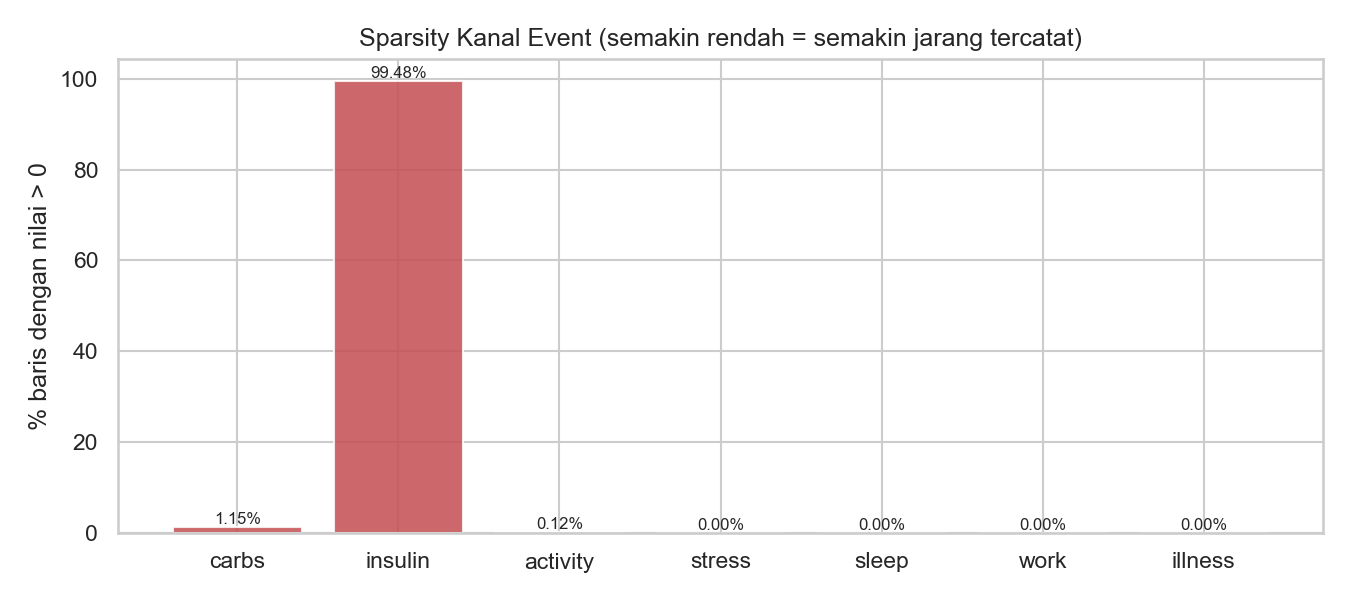
\includegraphics[width=0.92\textwidth]{images/Gambar_III3_SparsityKanal.png}
\caption{Proporsi baris dengan nilai lebih besar dari nol pada setiap kanal kejadian dataset OhioT1DM.}
\label{fig:sparsity-kanal}
\end{figure}

Gambar~\ref{fig:sparsity-kanal} memperlihatkan tiga pola yang masing-masing berujung pada satu keputusan rancangan. Pertama, kanal \texttt{carbs} hanya terisi pada 1,15\% baris, yang wajar bagi kejadian makan tiga sampai lima kali sehari, sehingga pemakaian nilai mentahnya akan membuat model kehilangan informasi pada 98,85\% titik waktu lainnya. Pola ini mendasari pemakaian besaran \emph{carbohydrate on board}. Kedua, kanal \texttt{insulin} justru terisi pada 99,48\% baris. Kerapatan itu bukan karena pemberian insulin berlangsung terus-menerus sebagai kejadian, melainkan karena kanal tersebut memuat laju basal yang diinfus tanpa henti. Komponen yang benar-benar bersifat sesaat adalah bolus, sehingga komponen itulah yang direpresentasikan sebagai \emph{insulin on board}, sebagaimana diuraikan pada Subbab~\ref{subsec:insulin}. Ketiga, kanal \texttt{stress}, \texttt{sleep}, \texttt{work}, dan \texttt{illness} praktis kosong, dengan proporsi yang membulat menjadi nol persen.

Variabel stres dikeluarkan dari himpunan fitur prediktor. Alasannya bersifat empiris, yaitu jumlah kejadian stres yang tercatat pada keseluruhan dataset terlalu sedikit untuk menghasilkan varians yang informatif. Variabel tersebut tetap dipertahankan sebagai bagian dari catatan \emph{logbook} karena relevansinya pada saat penerapan, sebagaimana didukung temuan \textcite{velasco2022} yang telah diuraikan pada Subbab~\ref{subsec:faktor-psikologis}.

\subsection{Analisis Horizon dan Skema Prediksi}
\label{subsec:horizon-prediksi}

Horizon prediksi ditetapkan pada 30 menit dan 60 menit. Penetapan ini bersandar pada dua dasar yang berdiri sendiri.

Dasar pertama bersifat klinis. Horizon prediksi tidak boleh lebih pendek daripada lingkar tindakan klinisnya. Setelah tatalaksana hipoglikemia awal diberikan, kadar glukosa darah diperiksa ulang dalam 15 menit, dan karbohidrat kerja cepat menaikkan kadar glukosa dalam rentang 10 hingga 15 menit setelah pemberian. Insulin analog kerja cepat memiliki awitan 5 hingga 15 menit dengan puncak kerja 30 hingga 90 menit \autocite{idai2015}. Dengan demikian, horizon 30 menit merupakan rentang terpendek yang masih menyisakan waktu untuk mengambil tindakan sekaligus memverifikasi hasilnya, sedangkan horizon 60 menit membentang tepat pada puncak kerja insulin kerja cepat, yaitu jendela ketika koreksi berlebihan berubah menjadi hipoglikemia.

Dasar kedua bersifat keterbandingan. Kedua horizon tersebut lazim digunakan pada penelitian prediksi glukosa di atas dataset OhioT1DM, sehingga hasil penelitian ini dapat disandingkan dengan penelitian terdahulu.

Horizon lima menit tidak digunakan meskipun sesuai dengan selang perekaman dataset. Alasannya bersifat ganda. Secara statistik, pada horizon sependek itu kadar glukosa nyaris tidak berubah sehingga tugas prediksi menjadi setara dengan menyalin nilai terakhir dan fitur multimoda tidak berkontribusi. Secara klinis, pada rentang tersebut belum ada tindakan apa pun yang sempat memberikan efek.

Horizon yang lebih panjang juga dipertimbangkan dan ditolak. Alasan penolakannya beserta bukti pengukurannya dibahas pada Bab~\ref{chap:evaluasi}.

Skema prediksi menggunakan prediksi langsung pada horizon tetap, bukan penggulungan rekursif banyak langkah. Pilihan ini menghindari akumulasi galat yang terjadi ketika keluaran suatu langkah dijadikan masukan langkah berikutnya.

Pembagian data latih dan data uji dilakukan per pasien, bukan per baris. Pembagian per baris akan menempatkan potongan deret waktu dari pasien yang sama pada kedua himpunan, sehingga model dapat memanfaatkan pola yang seharusnya belum dikenalnya. Penormalan fitur juga hanya disesuaikan pada data latih, dengan parameter yang sama diterapkan pada data uji.

\subsection{Kurasi Basis Pengetahuan}
\label{subsec:kurasi-kb}

Basis pengetahuan menentukan batas kemampuan sistem, karena rekomendasi yang dihasilkan tidak dapat melampaui isi dokumen yang tersedia untuk ditelusuri. Kurasi korpus karena itu diperlakukan sebagai keputusan rancangan tersendiri, bukan sebagai pengumpulan dokumen yang bersifat sekadarnya.

Kriteria yang digunakan pada penelitian ini disebut kriteria keterpicuan, yaitu sebuah topik hanya disertakan apabila dapat dipicu oleh variabel yang benar-benar teramati pada dataset penelitian. Kriteria ini menggantikan pendekatan yang mengumpulkan sebanyak mungkin dokumen pedoman, dengan dua alasan. Pertama, topik yang tidak dapat dipicu oleh variabel mana pun tidak akan pernah muncul pada hasil penelusuran, sehingga keberadaannya hanya menambah beban pengindeksan. Kedua, kriteria yang eksplisit memungkinkan cakupan korpus dinilai secara terukur, dan bukan berdasarkan penilaian yang bersifat pribadi.

Penerapan kriteria tersebut menghasilkan pemetaan dari variabel dataset ke topik pedoman sebagaimana disajikan pada Tabel~\ref{tab:pemetaan-variabel}.

\begin{longtable}{@{}p{4.4cm}p{4.2cm}p{5.4cm}@{}}
\caption{Pemetaan variabel dataset ke topik pedoman.}
\label{tab:pemetaan-variabel} \\
\toprule
\textbf{Variabel pada dataset} & \textbf{Kondisi yang dapat dipicu} & \textbf{Topik pedoman yang diperlukan} \\
\midrule
\endfirsthead

\multicolumn{3}{@{}l}{\small\emph{Tabel \thetable{} (lanjutan)}} \\
\toprule
\textbf{Variabel pada dataset} & \textbf{Kondisi yang dapat dipicu} & \textbf{Topik pedoman yang diperlukan} \\
\midrule
\endhead

\bottomrule
\endlastfoot

\texttt{glucose\_level}, \texttt{finger\_stick} & Kadar glukosa dalam atau di luar rentang sasaran & Pemantauan dan target glikemik \\[2pt]

\texttt{finger\_stick} rendah, \texttt{hypo\_event} & Hipoglikemia & Tata laksana hipoglikemia \\[2pt]

\texttt{glucose\_level} tinggi berkepanjangan & Hiperglikemia & Tata laksana hiperglikemia \\[2pt]

\texttt{glucose\_level} sangat tinggi & Risiko ketoasidosis & Ketoasidosis diabetik \\[2pt]

\texttt{bolus}, \texttt{basal}, \texttt{temp\_basal} & Penyesuaian dosis insulin & Terapi insulin \\[2pt]

\texttt{meal} beserta estimasi karbohidrat & Asupan karbohidrat & Nutrisi dan penghitungan karbohidrat \\[2pt]

\texttt{exercise}, \texttt{work} beserta intensitas & Aktivitas fisik & Pengelolaan saat aktivitas fisik \\[2pt]

\texttt{illness} & Kondisi sakit penyerta & Pengelolaan pada hari sakit \\[2pt]

\texttt{stressors} & Stres psikologis & Dipertahankan sebagai variabel \emph{logbook}, tidak dijadikan pemicu penelusuran karena jumlah kejadiannya terlalu sedikit \\

\end{longtable}

\noindent\footnotesize Pemetaan disusun melalui penelaahan kepadatan istilah kunci pada setiap dokumen korpus, kemudian divalidasi secara manual. Atribut durasi pada kanal \texttt{exercise} tidak diekstraksi, sehingga aktivitas fisik terwakili hanya oleh skor intensitas.\normalsize


Tabel~\ref{tab:pemetaan-variabel} memperlihatkan bahwa sembilan topik dapat dipicu oleh variabel yang tersedia, sedangkan sejumlah topik lain yang secara klinis penting tidak dapat dipicu karena variabel penandanya tidak terekam pada dataset. Topik yang dikecualikan beserta alasannya perlu dinyatakan secara terbuka. Topik puasa keagamaan dikecualikan karena proses penyamaran identitas pada dataset menggeser bulan pada seluruh catatan waktu, sehingga dokumentasi dataset menyatakan sendiri bahwa pengaruh musim maupun hari besar tidak dapat ditelaah \autocite{marling2020}. Topik kehamilan dikecualikan karena tidak terdapat penanda kehamilan pada dataset. Topik penapisan komplikasi dan penyakit penyerta dikecualikan karena tidak tersedia data laboratorium pendukung. Topik penentuan stadium DMT1 dikecualikan karena tidak tersedia data autoantibodi maupun kadar C-peptida.

Korpus yang dihasilkan dari penerapan kriteria tersebut terdiri atas dua belas dokumen dengan total 543 halaman, sebagaimana dirinci pada Tabel~\ref{tab:korpus-kb}. Dari jumlah itu, \textbf{494 halaman} yang benar-benar diindeks: 45 halaman depan berupa sampul, kata pengantar, dan daftar isi sengaja disaring karena padat kata kunci topik tanpa isi klinis sehingga mencemari hasil penelusuran, sedangkan 4 halaman lainnya berisi teks yang terlalu pendek untuk menghasilkan potongan bermakna. Angka 494 inilah yang menjadi dasar seluruh pengukuran penelusuran pada Bab~\ref{chap:evaluasi}.

\begin{longtable}{@{}p{1.5cm}p{4.6cm}p{1.1cm}p{1.5cm}p{5.0cm}@{}}
\caption{Korpus basis pengetahuan.}
\label{tab:korpus-kb} \\
\toprule
\textbf{Kode} & \textbf{Lembaga} & \textbf{Tahun} & \textbf{Halaman} & \textbf{Topik utama} \\
\midrule
\endfirsthead

\multicolumn{5}{@{}l}{\small\emph{Tabel \thetable{} (lanjutan)}} \\
\toprule
\textbf{Kode} & \textbf{Lembaga} & \textbf{Tahun} & \textbf{Halaman} & \textbf{Topik utama} \\
\midrule
\endhead

\bottomrule
\endlastfoot

KB-01 & IDAI UKK Endokrinologi Anak dan Remaja & 2015 & 129 & Hipoglikemia, insulin \\
KB-02 & PERKENI & 2021 & 49 & Pemantauan, insulin \\
KB-03 & PERKENI & 2021 & 70 & Insulin \\
KB-04 & PERKENI & 2023 & 105 & Hiperglikemia, insulin \\
KB-05 & ADA dan EASD & 2021 & 44 & Hipoglikemia, insulin, target glikemik \\
KB-06 & Konsensus Internasional ATTD & 2019 & 11 & Pemantauan, target glikemik \\
KB-07 & ISPAD Bab 10 & 2022 & 25 & Karbohidrat, insulin \\
KB-08 & ISPAD Bab 11 & 2022 & 22 & Ketoasidosis, insulin \\
KB-09 & ISPAD Bab 12 & 2022 & 19 & Hipoglikemia, insulin \\
KB-10 & ISPAD Bab 13 & 2022 & 14 & Ketoasidosis, insulin, hari sakit \\
KB-11 & ISPAD Bab 14 & 2022 & 32 & Aktivitas, karbohidrat, hipoglikemia \\
KB-12 & ISPAD Bab 25 & 2022 & 23 & Insulin, penyesuaian tata laksana pada keterbatasan sumber daya, bersifat lintas kondisi \\
\midrule
& \textbf{Total} & & \textbf{543} & \\

\end{longtable}

\noindent\footnotesize Judul lengkap setiap dokumen disajikan pada Lampiran. Kolom topik utama disarikan dari manifes korpus, yang memuat pula nilai penyeimbang nomor halaman untuk keperluan keterlacakan sitasi sebagaimana dituntut KNF-08.\normalsize


Tabel~\ref{tab:korpus-kb} memperlihatkan komposisi yang disengaja, yaitu empat dokumen berkonteks Indonesia untuk memastikan keselarasan dengan ketersediaan terapi setempat, dua konsensus internasional untuk DMT1 dewasa yang sesuai dengan rentang usia kontributor dataset, serta enam bab pedoman ISPAD yang menyediakan tata laksana spesifik per kondisi. Satu dokumen pada korpus tersebut, yaitu KB-12 mengenai pengelolaan pada lingkungan dengan sumber daya terbatas, disertakan atas dasar yang berbeda dari kriteria keterpicuan. Dokumen tersebut tidak memuat tata laksana yang terikat pada satu kondisi tertentu, melainkan pertimbangan penyesuaian tata laksana ketika ketersediaan perangkat dan obat terbatas. Perannya karena itu bersifat lintas kondisi, yaitu melengkapi dokumen lain ketika tata laksana baku tidak dapat dijalankan sepenuhnya. Dokumen ini tidak dipetakan pada Tabel~\ref{tab:pemetaan-variabel} karena tidak dipicu oleh variabel tunggal mana pun. Penyertaannya dinyatakan secara terbuka agar penerapan kriteria keterpicuan tetap konsisten.

Dua keterbatasan pada korpus tersebut perlu dinyatakan. Pertama, keenam bab ISPAD ditujukan bagi anak dan remaja, sedangkan kontributor dataset seluruhnya berusia dewasa. Bab-bab tersebut tetap disertakan karena isi operasionalnya, seperti ambang penanganan hipoglikemia dan aturan pengelolaan pada hari sakit, sebagian besar tidak bergantung pada usia, dan karena tidak tersedia padanan berbahasa Indonesia untuk topik-topik tersebut. Kedua, pemetaan topik pada Tabel~\ref{tab:pemetaan-variabel} disusun melalui penelaahan kepadatan istilah pada setiap dokumen, kemudian divalidasi secara manual. Pendekatan leksikal tersebut dapat melewatkan pembahasan yang menggunakan istilah berbeda, sehingga validasi manual menjadi bagian yang tidak terpisahkan dari prosedurnya.

\section{Analisis Pemilihan Solusi}
\label{sec:pemilihan-solusi}

\subsection{Alternatif Solusi}
\label{subsec:alternatif-solusi}

Untuk setiap keputusan rancangan utama dipertimbangkan sejumlah alternatif konkret sebagai berikut.

\begin{enumerate}
    \item \textbf{Model prediksi.} \emph{Random Forest}, \emph{Long Short-Term Memory}, atau \emph{Gradient Boosting Machine}.
    \item \textbf{Model bahasa.} Layanan awan Google Gemini atau model lokal yang dijalankan melalui Ollama.
    \item \textbf{Model \emph{embedding}.} Model \emph{sentence-transformers} yang dijalankan secara lokal, layanan \emph{embedding} berbasis awan, atau model \emph{embedding} lokal melalui Ollama.
    \item \textbf{Kerangka antarmuka.} Streamlit, Gradio, atau kerangka aplikasi web umum.
    \item \textbf{Skema pengambilan pengetahuan.} Penelusuran berbasis RAG di atas korpus dokumen tak terstruktur, atau penelusuran SPARQL di atas graf pengetahuan sebagaimana pendekatan \textcite{rad2024}.
    \item \textbf{Pengklasifikasi kondisi.} Penetapan ambang langsung atas nilai keluaran regresi, atau pengklasifikasi terpisah yang dilatih khusus untuk mengenali kondisi.
    \item \textbf{Orkestrasi alur.} Penulisan alur sebagai kode program, atau perangkaian melalui perkakas alur kerja visual.
\end{enumerate}

\subsection{Analisis Penentuan Solusi}
\label{subsec:penentuan-solusi}

Penentuan solusi dilakukan melalui dua langkah. Langkah pertama menilai setiap alternatif terhadap kebutuhan yang telah ditetapkan pada Subbab~\ref{sec:kebutuhan-sistem}, sebagaimana disajikan pada matriks Tabel~\ref{tab:matriks-solusi}.

% =====================================================================
% BELUM LENGKAP - PERLU DIISI SETELAH BAB VI SELESAI
%
% 1. Kolom penilaian hanya boleh diisi setelah angka evaluasi final
%    tersedia pada Bab VI.
% 2. Kelompok "Model prediksi" TERTAHAN sampai keputusan pembimbing
%    mengenai Random Forest atau Gradient Boosting ditetapkan.
%    Rujukan: docs/ALUR_SISTEM_FINAL.md dan docs/KEPUTUSAN_DIAMBIL.md
%
% Legenda: ++ memenuhi penuh | + memenuhi | o memenuhi sebagian
%          -  tidak memenuhi | * alternatif yang dipilih
%
% Catatan teknis: tabel ini sengaja TIDAK memakai \multirow karena
% paket multirow belum dimuat pada TA.tex. Nama keputusan ditulis pada
% baris pertama tiap kelompok, baris berikutnya dikosongkan.
% =====================================================================
\begin{longtable}{@{}p{2.5cm}p{3.2cm}p{1.1cm}p{1.1cm}p{1.15cm}p{1.2cm}p{1.1cm}@{}}
\caption{Matriks penilaian alternatif terhadap kebutuhan.}
\label{tab:matriks-solusi} \\
\toprule
\textbf{Keputusan} & \textbf{Alternatif} & \textbf{KNF-01} & \textbf{KNF-02} & \textbf{Ketepat.} & \textbf{Determin.} & \textbf{Bukti VI} \\
\midrule
\endfirsthead

\multicolumn{7}{@{}l}{\small\emph{Tabel \thetable{} (lanjutan)}} \\
\toprule
\textbf{Keputusan} & \textbf{Alternatif} & \textbf{KNF-01} & \textbf{KNF-02} & \textbf{Ketepat.} & \textbf{Determin.} & \textbf{Bukti VI} \\
\midrule
\endhead

\bottomrule
\endlastfoot

Model prediksi & Random Forest             & & & & & \\
               & Long Short-Term Memory    & & & & & \\
               & Gradient Boosting Machine & & & & & \\
\midrule

Model bahasa & Layanan awan & & & & & \\
             & Model lokal  & & & & & \\
\midrule

Model \emph{embedding} & \emph{sentence-transformers} lokal & & & & & \\
                       & Layanan \emph{embedding} awan      & & & & & \\
                       & \emph{Embedding} lokal via Ollama  & & & & & \\
\midrule

Kerangka antarmuka & Streamlit         & & & & & \\
                   & Gradio            & & & & & \\
                   & Kerangka web umum & & & & & \\
\midrule

Skema pengambilan & RAG atas korpus tak terstruktur & & & & & \\
pengetahuan       & SPARQL atas graf pengetahuan    & & & & & \\
\midrule

Pengklasifikasi & Ambang atas nilai regresi & & & & & \\
kondisi         & Pengklasifikasi terpisah  & & & & & \\
\midrule

Orkestrasi alur & Penulisan sebagai kode program & & & & & \\
                & Perkakas alur kerja visual     & & & & & \\

\end{longtable}

\noindent\footnotesize Legenda: $++$ memenuhi penuh, $+$ memenuhi, $\circ$ memenuhi sebagian, $-$ tidak memenuhi, dan $\bullet$ menandai alternatif yang dipilih. Kolom ketepat.\ mengacu pada ketepatan fungsional, kolom determin.\ mengacu pada sifat deterministik keluaran, dan kolom bukti VI mengacu pada ketersediaan bukti empiris pada Bab~\ref{chap:evaluasi}.\normalsize


Tabel~\ref{tab:matriks-solusi} menegaskan bahwa keputusan rancangan diturunkan dari kebutuhan dan bukan dari preferensi, karena setiap sel dapat ditelusuri ke kebutuhan yang bersangkutan. Perlu dicatat bahwa matriks tersebut bukan sekadar dokumentasi atas keputusan yang telah diambil sejak awal. Salah satu barisnya, yaitu pengklasifikasi kondisi, justru merupakan keputusan yang berubah setelah bukti empiris diperoleh. Penetapan ambang langsung atas nilai keluaran regresi semula digunakan, kemudian ditinggalkan setelah terbukti hanya menangkap sebagian kecil kejadian hipoglikemia. Perubahan tersebut merupakan penerapan siklus DSRM sebagaimana dimaksud \textcite{peffers2007}, yaitu hasil evaluasi mengumpanbalik ke tahap perancangan.

Langkah kedua merangkum alasan pemilihan beserta kelemahan yang diakui pada setiap keputusan, sebagaimana disajikan pada Tabel~\ref{tab:penentuan-solusi}.

% =====================================================================
% BARIS "Model prediksi" TERTAHAN.
%
% Dua alasan lama - keterjelasan kontribusi fitur dan kebutuhan
% komputasi rendah - SUDAH DICABUT oleh KEPUTUSAN #5:
%   - keterjelasan  : digugurkan J7. Yang dimiliki RF secara bawaan
%                     adalah MDI, sedangkan MDI tidak boleh dilaporkan karena
%                     bias kardinalitas. Angka yang dilaporkan adalah
%                     permutation importance, yang MODEL-AGNOSTIK.
%   - komputasi     : terbalik secara faktual (RF paling mahal).
%
% Isi baris tersebut setelah keputusan Random Forest atau Gradient
% Boosting ditetapkan. Rujukan: docs/KEPUTUSAN_DIAMBIL.md,
% docs/ALUR_SISTEM_FINAL.md, docs/REVISI_BAB_II_4_1.md.
% =====================================================================
\begin{longtable}{@{}p{2.5cm}p{2.7cm}p{3.8cm}p{3.6cm}@{}}
\caption{Alasan pemilihan dan kelemahan yang diakui.}
\label{tab:penentuan-solusi} \\
\toprule
\textbf{Keputusan} & \textbf{Alternatif terpilih} & \textbf{Alasan pemilihan} & \textbf{Kelemahan yang diakui} \\
\midrule
\endfirsthead

\multicolumn{4}{@{}l}{\small\emph{Tabel \thetable{} (lanjutan)}} \\
\toprule
\textbf{Keputusan} & \textbf{Alternatif terpilih} & \textbf{Alasan pemilihan} & \textbf{Kelemahan yang diakui} \\
\midrule
\endhead

\bottomrule
\endlastfoot

Model prediksi & \emph{Gradient Boosting} & Kriteria pemilihannya akurasi kelas kondisi, bukan galat regresi, sebab kelas kondisi itulah yang menyusun kueri penelusuran; pada kriteria tersebut ia unggul, sementara galat regresinya setara & Kepekaan terhadap hipoglikemia pada horizon 60~menit lebih rendah daripada \emph{Random Forest}, dan pengklasifikasinya menukar ketepatan demi kepekaan \\[2pt]

Model bahasa & Layanan awan & Tidak membebani perangkat lokal dan tersedia berjenjang gratis & Memerlukan konektivitas jaringan sebagaimana Batasan~5 \\[2pt]

Model \emph{embedding} & \emph{sentence-transformers} lokal & Berjalan tanpa akselerator grafis dan tanpa biaya per permintaan & Keterbatasan pada penelusuran lintas bahasa sebagaimana Subbab~\ref{subsec:arsitektur-rag} \\[2pt]

Kerangka antarmuka & Streamlit & Pengembangan cepat untuk purwarupa dan integrasi langsung dengan ekosistem Python & Keterbatasan penyesuaian tata letak untuk kebutuhan lanjutan \\[2pt]

Skema pengambilan pengetahuan & RAG di atas korpus tak terstruktur & Tidak menuntut pembangunan ontologi maupun integrasi rekam medis & Mutu bergantung pada cakupan korpus \\[2pt]

Pengklasifikasi kondisi & Pengklasifikasi terpisah & Terbukti menangkap kejadian hipoglikemia jauh lebih baik daripada penetapan ambang atas nilai regresi & Menambah satu model yang perlu dilatih dan dipelihara, serta menurunkan nilai duga positif \\[2pt]

Orkestrasi alur & Penulisan sebagai kode program & Memenuhi pemisahan logika domain (KNF-07) dan berjalan tanpa server khusus (KNF-09) & Menuntut penulisan kode yang lebih banyak dibandingkan perkakas visual \\

\end{longtable}


Tabel~\ref{tab:penentuan-solusi} menyertakan kolom kelemahan secara sengaja, karena tidak terdapat alternatif yang unggul pada seluruh kriteria, sehingga setiap pemilihan merupakan pertukaran yang perlu dinyatakan secara terbuka.

\subsection{Gambaran Umum Solusi Terpilih}
\label{subsec:gambaran-umum-solusi}

Hasil analisis pada subbab sebelumnya menghasilkan rancangan sistem yang alurnya digambarkan secara umum pada Gambar~\ref{fig:gambaran-umum-sistem}.

\begin{figure}[htbp]
\centering
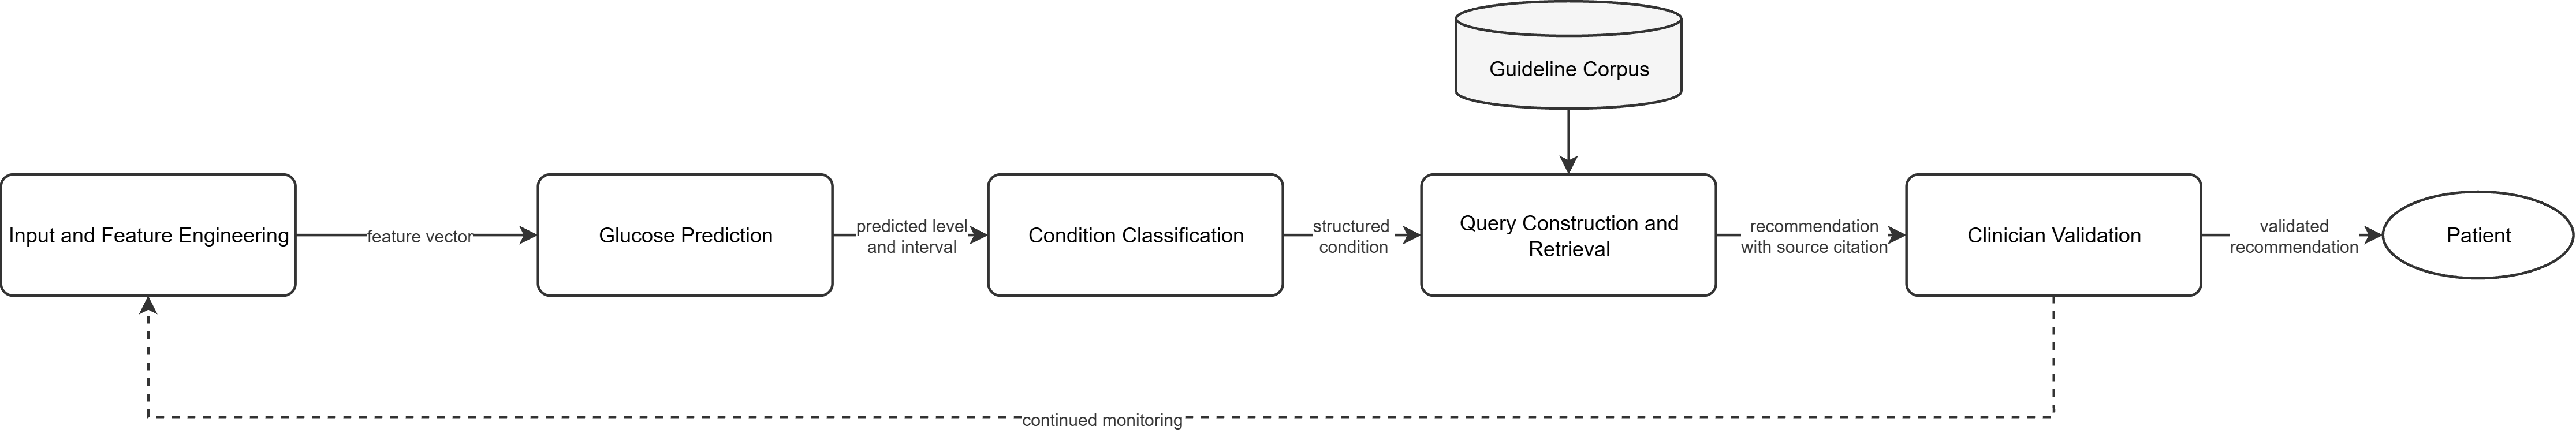
\includegraphics[width=\textwidth]{images/Gambar_III2_GambaranUmumSistem.png}
\caption{Gambaran umum alur sistem yang diusulkan.}
\label{fig:gambaran-umum-sistem}
\end{figure}

Gambar~\ref{fig:gambaran-umum-sistem} memperlihatkan bahwa sistem bekerja dalam lima tahap yang berurutan. Tahap pertama menerima catatan \emph{logbook} dan mengubahnya menjadi vektor fitur melalui rekayasa fitur, mencakup perhitungan besaran \emph{insulin on board} dan \emph{carbohydrate on board} sebagaimana diuraikan pada Subbab~\ref{subsec:pemilihan-fitur}. Tahap kedua menghasilkan taksiran kadar glukosa pada horizon 30 dan 60 menit beserta selang ketidakpastiannya. Tahap ketiga menerjemahkan taksiran tersebut menjadi kondisi klinis terstruktur berupa tingkat risiko, arah perubahan, dan tingkat kegentingan. Tahap keempat menyusun kueri penelusuran dari kondisi terstruktur tersebut, lalu menelusuri korpus pedoman dan menyusun rekomendasi berbahasa Indonesia yang disertai penunjuk dokumen dan halaman sumbernya. Tahap kelima menyerahkan rekomendasi kepada dokter untuk divalidasi sebelum diteruskan kepada pasien.

Perbedaan pokok terhadap sistem berbasis RAG pada umumnya terletak pada tahap keempat. Pada sistem yang lazim, kueri penelusuran disusun dari kondisi yang sedang berlaku atau dari pertanyaan pengguna, sehingga panduan yang diperoleh menanggapi keadaan yang telah teramati. Pada sistem yang diusulkan, kueri disusun dari keluaran tahap ketiga, yaitu kondisi yang diperkirakan akan terjadi. Strategi inilah yang disebut \emph{query transformation} terkondisi-prediksi sebagaimana diperkenalkan pada Subbab~\ref{sec:kontribusi-penelitian}, sedangkan realisasinya menjadi pemenuhan KF-04 pada Tabel~\ref{tab:kebutuhan-fungsional}. Rancangan rinci setiap tahap beserta antarmuka antarmodulnya dipaparkan pada Bab~\ref{chap:perancangan}.
